
\section{Discrete data}

\subsection{Binary data} \label{sec:toenail}

\monolix~3.0 can now be used to estimate the parameters of a model where the outcome is a discrete response. The most simple of this, but also the least informative type, is a binary response that can take the values 0 or 1. In this section, we illustrate the use of \monolix to model binary data from a randomised clinical trial comparing two treatments for fungal toenail infection. We use the {\sf toenail} dataset available in {\sf R} in the packages {\sf prLogistic} or {\sf HSAUR3}.

Data are from \cite{debacker_toenail}, a multi-center randomised comparison  of two oral treatments (A and B) for toenail infection. 294 patients are measured at seven visits, i.e. at baseline (week 0), and at weeks 4, 8, 12, 24, 36, and 48 thereafter, comprising a total of 1908 measurements. The primary end point was the absence of toenail infection and the outcome of interest is the binary variable "onycholysis" which indicates the degree of separation of the nail plate from the nail-bed (categorised as 0=none or mild versus 1=moderate or severe). Figure~\ref{fig:toenailData} shows the evolution of the number of events (left) and the proportion of events (right) in the two treatment groups over the 7 visits of the study.

\begin{figure}[!h]
\begin{center}
\epsfig{file=figs/toenail_barplotData.eps,width=7.5cm,angle=0}
\epsfig{file=figs/toenail_rawdata.eps,width=7.5cm,angle=0}
\end{center}
\par \kern -0.5cm
\caption{Toenail data. Left: number of events at each visit; right: proportion of infected subjects at each visit.} \label{fig:toenailData}
\end{figure}

Several analyses have been made in the literature \cite{lesaffre2001effect,lin2011goodness}, and here we fit the logistic random effect model developed by \cite{hedeker1994random}. This model includes a random intercept ($\theta_1$, normally distributed with a standard deviation $\omega_1$),  a time effect ($\beta_2$, normally distributed with a standard deviation $\omega_2$). Treatment (A or B) ($\beta$) is included as a covariate on time. The treatments were randomised at baseline so we don't include a treatment effect on the intercept. The probability $p_{ij}=P(Y_{ij}=1 | \theta_{1,i}, \theta_{2,i})$ associated with an event $Y_{ij}$ at time $t_{ij}$ is given by the following equation for the logit:
\begin{equation}
logit(p_{ij}) = \ln \left( \frac{p_{ij}}{1-p_{ij}} \right) = \theta_{1,i} + \theta_{1,i} t_{ij} \label{eq:logit}
\end{equation}

For non-gaussian models, the model function must be written to return the log-pdf, that is, the logarithm of the probability of the observed response given a set of parameters. To do this we need to pass the response as one of the predictors when creating the {\sf SaemixData} object.
\begin{verbatim}
data(toenail.saemix)
saemix.data<-saemixData(name.data=toe,name.group=c("id"),name.predictors=c("time","y"), 
    name.response="y", name.covariates=c("treatment"),name.X=c("time"))
\end{verbatim}

The model function can now be written. As previously, it must take 3 arguments, {\sf psi}, {\sf id} and {\sf xidep}. Within the body of the function, we compute the logpdf as a function of the parameters. Here for a binomial model, this means we define first the logit of the probability, then the probability itself by inverting equation~\ref{eq:logit}. We then define the probability of the observed outcome as $pevent \; \mathbb{1}_{Y=1} + (1-pevent) \; \mathbb{1}_{Y=0}$
\begin{verbatim}
binary.model<-function(psi,id,xidep) {
  tim<-xidep[,1]
  y<-xidep[,2]
  inter<-psi[id,1]
  slope<-psi[id,2]
  logit<-inter+slope*tim
  pevent<-exp(logit)/(1+exp(logit))
  pobs = (y==0)*(1-pevent)+(y==1)*pevent
  logpdf <- log(pobs)
  return(logpdf)
}
\end{verbatim}

We can also add a simulation function to the model definition, which we will use later to obtain diagnostics. This simulation function has the same structure as the model function, but after defining the probability $pevent$, we use it to simulate from a binomial model. This function is not required for fitting, but is necessary to be able to use the simulation function we will define later. Notice the similarity with the model function {\sf binary.model} defined above: we replaced the line defining the log-probability {\sf logp} in {\sf binary.model}  call to the {\sf rbinom} function from {\sf R} to obtain simulations from a Bernouilli distribution with probability $pevent$ for each value of time, and we return those simulated events.
\begin{verbatim}
simulBinary<-function(psi,id,xidep) {
  tim<-xidep[,1]
  y<-xidep[,2]
  inter<-psi[id,1]
  slope<-psi[id,2]
  logit<-inter+slope*tim
  pevent<-1/(1+exp(-logit))
  ysim<-rbinom(length(tim),size=1, prob=pevent)
  return(ysim)
}
\end{verbatim}

To tell \monolix~that we are now dealing with non-continuous responses, we add the argument {\sf modeltype='likelihood'} to the definition of the model using the function {\sf saemixModel}. We assume only the intercept has interindividual variability, and follows a normal distribution. We set the covariate model for a treatment effect on $\theta_2$. We pass the simulation function in the {\sf simulate.function} argument (optional).
\begin{verbatim}
saemix.model<-saemixModel(model=binary.model,description="Binary model",
    modeltype="likelihood", simulate.function=simulBinary,
    psi0=matrix(c(-5,-.1,0,0),ncol=2,byrow=TRUE,dimnames=list(NULL,
    c("theta1","theta2"))),
    transform.par=c(0,0), covariate.model=c(0,1),
    covariance.model=matrix(c(1,0,0,0),ncol=2))
\end{verbatim}

We then fit the model, setting the option {\sf fim=FALSE} as the approximation used in the computation of the FIM by linearisation is not appropriate in discrete models. Since binary data contains very limited information, it is advised to increase the number of chains to stabilise the estimation. Here we set the number of chains to 10.
\begin{verbatim}
saemix.options<-list(seed=1234567,save=FALSE,save.graphs=FALSE, 
    displayProgress=FALSE, nb.chains=10, fim=FALSE)
binary.fit<-saemix(saemix.model,saemix.data,saemix.options)
\end{verbatim}

{\bf Important note:} The linear approximation of the FIM does not apply well to discrete response models. Exact computation methods to estimate the FIM without linearisation have been proposed by~\cite{Riviere16} using Hamiltonian Monte-Carlo and~\cite{Ueckert16} using adaptive Gaussian quadrature. These methods can be applied to estimate SE for the parameters but are not automatically available yet in \monolix.

\paragraph{Diagnostics:} automated visualisation or diagnostic plots have not yet been implemented for discrete response models, but we can of course create our own in R by simulating from the model. The {\sf simulateDiscreteSaemix} function uses the model fit and the simulation function (defined above) to simulate responses from the estimated parameter distribution.
% ECO TODO: add Marc's npd for categorical data...
\begin{verbatim}
nsim<-100
binary.fit <- simulateDiscreteSaemix(binary.fit, nsim=nsim)
\end{verbatim}

In figure~\ref{fig:toenailPropVPC} we use the simulated data in the {\sf datasim} dataframe contained in the {\sf sim.data} element of the object after the call to the function to compute a 90\% prediction interval on the proportion of events at each visit. This VPC plot shows a reasonable model fit in the two treatment groups.

\begin{figure}[!h]
\begin{center}
\epsfig{file=figs/toenail_globalVPC.eps,width=11cm,angle=0}
\end{center}
\par \kern -0.5cm
\caption{Proportion of expected events compared to the observed proportion across time, for the model fit to the toenail data.} \label{fig:toenailPropVPC}
\end{figure}

The following code was used to produce this plot (the libraries {\sf tidyverse, ggplot2} and {\sf gridExtra} are assumed to be loaded in the {\sf R} session):
\begin{verbatim}
simdat <-binary.fit@sim.data@datasim
simdat$visit<-rep(toenail.saemix$visit,nsim)
simdat$treatment<-rep(toenail.saemix$treatment,nsim)
 
# requires 
# library(tidyverse)
# library(ggplot2)
# library(gridExtra)

ytab<-NULL
for(irep in 1:nsim) {
  xtab<-simdat[simdat$irep==irep,]
  xtab1 <- xtab %>%
    group_by(visit, treatment) %>%
    summarise(nev = sum(ysim), n=n()) %>%
    mutate(freq = nev/n)
  ytab<-rbind(ytab,xtab1[,c("visit","freq","treatment")])
}
gtab <- ytab %>%
  group_by(visit, treatment) %>%
  summarise(lower=quantile(freq, c(0.05)), median=quantile(freq, c(0.5)), 
  upper=quantile(freq, c(0.95))) %>%
  mutate(treatment=ifelse(treatment==1,"B","A"))
gtab$freq<-1

# summarising data
toe1 <- toenail.saemix %>%
  group_by(visit, treatment) %>%
  summarise(nev = sum(y), n=n()) %>%
  mutate(freq = nev/n, sd=sqrt((1-nev/n)/nev)) %>%
  mutate(treatment=ifelse(treatment==1,"B","A"))

plot2 <- ggplot(toe1, aes(x=visit, y=freq, group=treatment)) + 
  geom_line(aes(colour=treatment)) + 
  geom_point(aes(colour=treatment)) + 
  geom_line(data=gtab, aes(x=visit, y=median), linetype=2, colour='lightblue') + 
  geom_ribbon(data=gtab,aes(ymin=lower, ymax=upper), alpha=0.5, fill='lightblue') +
  ylim(c(0,0.5)) + theme_bw() + theme(legend.position = "none") + 
  facet_wrap(.~treatment) +
  xlab("Visit number") + ylab("Frequency of infection")
print(plot2)
\end{verbatim}


\clearpage
\newpage

\subsection{Categorical data} \label{sec:kneeCat}

The {\sf knee.saemix} data represents pain scores recorded in a clinical study in 127 patients with sport related injuries treated with two different therapies. The pain occuring during knee movement was observed after 3,7 and 10 days of treatment. It was taken from the {\sf catdata} package in R~\cite{catdata} (dataset {\sf knee}) and reformatted as follows. A time column was added representing the day of the measurement (with 0 being the baseline value) and each observation corresponds to a different line in the dataset. Treatment was recoded as 0/1 (placebo/treatment), gender as 0/1 (male/female) and {\sf Age2} represents the squared of centered Age. Figure~\ref{fig:kneeData} shows barplots of the different pain scores as a function of time in study, illustrating a recovery as the proportion of lower pain scores increases.

\begin{figure}[!h]
\begin{center}
\epsfig{file=figs/knee_barplotData.eps,width=11cm,angle=0}
\end{center}
\par \kern -0.5cm
\caption{Barplot of the evolution of pain scores with time in the {\sf knee.saemix} dataset.} \label{fig:kneeData}
\end{figure}

\begin{verbatim}
data(knee.saemix)
\end{verbatim}

The dataset is part of the datasets analysed in~\cite{Tutz12} with various methods (please refer to the different vignettes in the documentation of {\sf knee}), but mainly as logistic regression on the response after 10 days, or as mixed binary regression after dichotomising the response. Here, we will fit the following proportional odds model to the full data:
The probability $p_{ij}=P(Y_{ij}=1 | \theta_{1,i}, \theta_{2,i})$ associated with an event $Y_{ij}$ at time $t_{ij}$ is given by the following equation for the logit:
\begin{equation}
\begin{split}
logit(P(Y_{ij} = 1 | \psi_i)) &= \alpha_{1,i} + \beta_{i} t_{ij} \\
logit(P(Y_{ij} = 2 | \psi_i)) &= \alpha_{1,i} + \alpha_2 \\
logit(P(Y_{ij} = 3 | \psi_i)) &= \alpha_{1,i} + \alpha_2 + \alpha_3 \\
logit(P(Y_{ij} = 4 | \psi_i)) &= \alpha_{1,i} + \alpha_2 + \alpha_3 +\alpha_4\\
P(Y_{ij} = 4 | \psi_i) &= 1 - \sum_k=1^4 P(Y_{ij} = k | \psi_i)\\
\end{split}
\end{equation}
where $\alpha_1$ and $\beta$ have interindividual variability, $\beta$ is the effect of time, $\alpha_1$ is the probability of a pain score of 1 and the other parameters represent an incremental risk to move into the higher pain category.

When the response has more than one category, we define the probability for (K-1) categories and combine them to obtain the likelihood for each observation.

\begin{verbatim}
ordinal.model<-function(psi,id,xidep) {
  y<-xidep[,1]
  time<-xidep[,2]
  alp1<-psi[id,1]
  alp2<-psi[id,2]
  alp3<-psi[id,3]
  alp4<-psi[id,4]
  beta<-psi[id,5]
  
  logit1<-alp1 + beta*time
  logit2<-logit1+alp2
  logit3<-logit2+alp3
  logit4<-logit3+alp4
  pge1<-exp(logit1)/(1+exp(logit1))
  pge2<-exp(logit2)/(1+exp(logit2))
  pge3<-exp(logit3)/(1+exp(logit3))
  pge4<-exp(logit4)/(1+exp(logit4))
  pobs<-(y==1)*pge1+(y==2)*(pge2-pge1)+(y==3)*(pge3-pge2)+(y==4)*(pge4-pge3)+(y==5)*(1-pge4)
  logpdf <- log(pobs)  
  return(logpdf)
}  
saemix.model<-saemixModel(model=ordinal.model,
        description="Ordinal categorical model",modeltype="likelihood",
        psi0=matrix(c(0,0.2, 0.6, 3, 0.2),ncol=5,byrow=TRUE,
           dimnames=list(NULL,c("alp1","alp2","alp3","alp4","beta"))),
        transform.par=c(0,1,1,1,1),
        covariance.model = diag(c(1,0,0,0,1)))

saemix.options<-list(seed=632545,save=FALSE,save.graphs=FALSE, nb.chains=10, 
    fim=FALSE)

ord.fit<-saemix(saemix.model,saemix.data,saemix.options)
\end{verbatim}

Figure~\ref{fig:kneeMedScoreVPC}, representing a VPC of the mean value of pain score at each time point, stratified over treatment, shows some model misfit especially for treatment 0. This figure was produced using simulations from the fitted model as in the binary data examples using the simulation function below.
\begin{figure}[!h]
\begin{center}
\epsfig{file=figs/knee_medianScoreVPC.eps,width=11cm,angle=0}
\end{center}
\par \kern -0.5cm
\caption{VPC of the mean value of pain score in the model adjusted to the {\sf knee.saemix} dataset.} \label{fig:kneeMedScoreVPC}
\end{figure}

\begin{verbatim}
simulateOrdinal<-function(psi,id,xidep) {
  y<-xidep[,1]
  time<-xidep[,2]
  alp1<-psi[id,1]
  alp2<-psi[id,2]
  alp3<-psi[id,3]
  alp4<-psi[id,4]
  beta<-psi[id,5]
  
  logit1<-alp1 + beta*time
  logit2<-logit1+alp2
  logit3<-logit2+alp3
  logit4<-logit3+alp4
  pge1<-exp(logit1)/(1+exp(logit1))
  pge2<-exp(logit2)/(1+exp(logit2))
  pge3<-exp(logit3)/(1+exp(logit3))
  pge4<-exp(logit4)/(1+exp(logit4))
  x<-runif(length(time))
  ysim<-1+as.integer(x>pge1)+as.integer(x>pge2)+as.integer(x>pge3)+as.integer(x>pge4)
  return(ysim)
}
\end{verbatim}


\subsection{Count data} 

\subsubsection{Epilepsy data} \label{sec:epilepsyCount}

We first show a simple example using the {\sf epilepsy} data from the {\sf MASS} package. We can fit the Poisson model to the data, which assumes that the probability to observe a count value equal to $n$ is given by:
\begin{equation}
P(Y=n) = \frac{\lambda^n \; e^{-\lambda}}{n!}
\end{equation}

where $\lambda>0$ is the parameter of the model. We assume a log-normal distribution for $\lambda$.

\begin{verbatim}
epilepsy<-MASS::epil
saemix.data<-saemixData(name.data=epilepsy, name.group=c("subject"),
     name.predictors=c("period","y"),name.response=c("y"),
     name.covariates=c("trt","base", "age"), 
     units=list(x="2-week",y="", covariates=c("","","yr")))
## Poisson model with one parameter
countPoi<-function(psi,id,xidep) { 
    y<-xidep[,2]
    lambda<-psi[id,1]
    logp <- -lambda + y*log(lambda) - log(factorial(y))
    return(logp)
    }
saemix.model<-saemixModel(model=countPoi,description="Count model Poisson",
   modeltype="likelihood", 
   psi0=matrix(c(0.5),ncol=1,byrow=TRUE,dimnames=list(NULL, c("lambda"))), 
   transform.par=c(1))
saemix.options<-list(seed=632545,save=FALSE,save.graphs=FALSE, 
   displayProgress=FALSE)
poisson.fit<-saemix(saemix.model,saemix.data,saemix.options)
\end{verbatim}

\subsubsection{RAPI data} \label{sec:RAPICount}

%Web-based brief alcohol interventions have the potential to reach a large number of individuals at low cost; however, few controlled evaluations have been conducted to date. The present study was designed to evaluate the efficacy of gender-specific versus gender-nonspecific personalized normative feedback (PNF) with single versus biannual administration in a 2-year randomized controlled trial targeting a large sample of heavy-drinking college students.

This dataset was kindly made available by David Atkins (University of Washington) in his tutorial on modelling count data~\cite{Atkins13} and comes from a randomised controlled trial assessing the effectiveness of web-based personalised normative feedback intervention on alcohol consumption~\cite{Neighbors10a, Neighbors10b}. The {\sf RAPI dataset} records alcohol-related problems, as measured by the Rutgers Alcohol Problem Index (RAPI)~\cite{White89}, in freshmen at risk for heavy drinking behaviours. Students were asked to report every six months the number of alcohol-related problems, and the dataset includes 3,616 repeated measures of these counts in 818 subjects, 561 of whom had the full 5 measurements over a period of 2 years. Interesting features of this dataset are first, the longitudinal aspect which allow to evaluate changes over time, and second, the shape of the distribution of counts. Counts are often positively skewed, bounded by zero, with a large stack of data points at zero, indicating individuals and/or occasions without drinking, use, or related problems. This dataset was used in~\cite{Atkins13} to illustrate mixed effects count regression using the {\sf glmer()} function from the {\sf lme4} package.

The dataset is available in \monolix~under the name {\sf rapi.saemix} so we read it and create our saemixData object in the usual way. Because we need the value of the outcome to compute the corresponding likelihood, the {\sf rapi} column is used both as a predictor and as the response:
\begin{verbatim}
data(rapi.saemix)
saemix.data<-saemixData(name.data=rapi.saemix, name.group=c("id"),
                 name.predictors=c("time","rapi"),name.response=c("rapi"),
                 name.covariates=c("gender"),
                 units=list(x="months",y="",covariates=c("")))
hist(rapi.saemix$rapi, main="", xlab="RAPI score", breaks=30)
\end{verbatim}
\monolix~currently does not have automated plots for discrete outcome data, but we can produce our own histogram (here, across all measurements without taking time into account) to notice that indeed, there seems to be many subjects reporting no alcohol related problems over some periods.

\paragraph{Poisson model:} the first model we can fit to this data is, as previously, the Poisson model, but this time we add a time effect. Here we will write the same model as in {\sf glmer()} to compare our results. In {\sf glmer()} a logarithmic link function is used to transform the mean of the Poisson model ($\lambda$) into a linear predictor of time and covariates. Random effects are then added to the parameters of the linear model. To take into account the change with time in {\sf saemix}, we need to rewrite the previous model to use normal distributions for the parameters and explicitely write the linear model in the function, as follows:
\begin{verbatim}
count.poisson<-function(psi,id,xidep) { 
  time<-xidep[,1]
  y<-xidep[,2]
  intercept<-psi[id,1]
  slope<-psi[id,2]
  lambda<- exp(intercept + slope*time)
  logp <- -lambda + y*log(lambda) - log(factorial(y))
  return(logp)
}
\end{verbatim}
The expression of logp in the model function is unchanged, but now we define a log-normal distribution for $\lambda$ within the model so that we can use two parameters and time as a predictor. The statistical model also changes to reflect this, as our parameters intercept and slope are now on the scale of the random effects, so they are given a normal distribution. 

Again we can define a simulation function associated with the model, with the same arguments as the model function, and returning simulated responses. For the Poisson model, this function would be the following, where we replace the line defining the log-probability {\sf logp} in {\sf count.poisson} with a line simulating from a Poisson distribution with parameter $\lambda$ for each value of time, and returning those simulated counts.
\begin{verbatim}
saemix.simulatePoisson<-function(psi, id, xidep) {
  time<-xidep[,1]
  y<-xidep[,2]
  intercept<-psi[id,1]
  slope<-psi[id,2]
  lambda<- exp(intercept + slope*time)
  y<-rpois(length(time), lambda=lambda)
  return(y)
}
\end{verbatim}

Defining and fitting this model in \monolix, we have:
\begin{verbatim}
saemix.model.poi<-saemixModel(model=count.poisson,description="Count model Poisson",
    modeltype="likelihood", simulate.function=saemix.simulatePoisson,
    psi0=matrix(c(log(5),0.01),ncol=2,byrow=TRUE,dimnames=list(NULL, c("intercept","slope"))), 
    transform.par=c(0,0), omega.init=diag(c(0.5, 0.5)))
saemix.options<-list(seed=632545,save=FALSE,save.graphs=FALSE, displayProgress=FALSE)
poisson.fit<-saemix(saemix.model.poi,saemix.data,saemix.options)
\end{verbatim}
Note that when parameters enter the model through a normal distribution, we may need to adjust the initial values of the $\Omega$ matrix (argument {\sf omega.init}) to avoid failure to find valid initial parameter estimates.

We can also add the covariate gender to both parameters as well as a correlation between the two random effects:
\begin{verbatim}
modsmx.poi.cov2<-saemixModel(model=count.poisson, simulate.function=saemix.simulatePoisson,
      description="Count model Poisson",modeltype="likelihood",   
      psi0=matrix(c(log(5),0.01),ncol=2,byrow=TRUE,dimnames=list(NULL, 
      c("intercept","slope"))), transform.par=c(0,0), 
      omega.init=diag(c(0.5, 0.5)), 
      covariance.model=matrix(data=1, ncol=2, nrow=2),
      covariate.model=matrix(c(1,1), ncol=2, byrow=TRUE))
poisson.fit.cov2<-saemix(modsmx.poi.cov2,saemix.data,saemix.options)
\end{verbatim}
Comparing the parameter estimates from this fit to the estimates obtained by {\sf glmer()} using a Laplace approximation in Table~2 of~\cite{Atkins13}, we find very good agreement with the SAEM algorithm.

\noindent{\bf Note:} \monolix~does not provide adequate standard errors of estimation for the parameters in version 3.0. The FO-approximation of the FIM implemented in the current version of the algorithm is known to be very poor for discrete outcome models.

Some diagnostics for this model can be obtained by simulating from the model. We use the {\sf simulateDiscreteSaemix} function to obtain simulations from the model, using the estimated parameters. Here we set the number of simulations to 100 as the dataset is large and we are interested in global diagnostics. Again 
\begin{verbatim}
yfit1<-simulateDiscreteSaemix(poisson.fit.cov2, nsim=100)
cat("Observed proportion of 0's", 
     length(yfit1@data@data$rapi[yfit1@data@data$rapi==0])/yfit1@data@ntot.obs,"\n")
cat("      Poisson model, p=",
    length(yfit1@sim.data@datasim$ysim[yfit1@sim.data@datasim$ysim==0])/
    length(yfit1@sim.data@datasim$ysim),"\n") 
\end{verbatim}

\paragraph{Handling overdispersion:} the model predicts a lower proportion of subjects without alcohol-related problems than we observe in data, a sign of overdispersion (with a Poisson model, the mean of the Poisson distribution, $\lambda$, is equal to the variance, an assumption which is violated here). Several models can be used to take this feature into account. First, we can use the Zero-Inflated Poisson model, where the number of counts equal to 0 is increased. This model can be built as a mixture between a distribution of 0's with probability $p_0$ and a standard Poisson model. We modify our model function above to:
\begin{verbatim}
count.poissonzip<-function(psi,id,xidep) {
  time<-xidep[,1]
  y<-xidep[,2]
  intercept<-psi[id,1]
  slope<-psi[id,2]
  p0<-psi[id,3] # Probability of zero's
  lambda<- exp(intercept + slope*time)
  logp <- log(1-p0) -lambda + y*log(lambda) - log(factorial(y)) # Poisson
  logp0 <- log(p0+(1-p0)*exp(-lambda)) # Zeroes
  logp[y==0]<-logp0[y==0]
  return(logp)
}
\end{verbatim}
as well as the associated simulation function:
\begin{verbatim}
saemix.simulatePoissonZIP<-function(psi, id, xidep) {
  time<-xidep[,1]
  y<-xidep[,2]
  intercept<-psi[id,1]
  slope<-psi[id,2]
  p0<-psi[id,3] # Probability of zero's
  lambda<- exp(intercept + slope*time)
  prob0<-rbinom(length(time), size=1, prob=p0)
  y<-rpois(length(time), lambda=lambda)
  y[prob0==1]<-0
  return(y)
}
\end{verbatim}
and fit the model using:
\begin{verbatim}
modsmx.zip<-saemixModel(model=count.poissonzip,description="count model ZIP",
   modeltype="likelihood", simulate.function=saemix.simulatePoissonZIP,
   psi0=matrix(c(1.5, 0.01, 0.2),ncol=3,byrow=TRUE,dimnames=list(NULL, 
      c("intercept", "slope","p0"))), 
   transform.par=c(0,0,3), covariance.model=diag(c(1,1,0)), 
   omega.init=diag(c(0.5,0.3,0)),
   covariate.model = matrix(c(1,1,0),ncol=3, byrow=TRUE))

zippoisson.fit <- saemix(modsmx.zip,saemix.data,saemix.options)
\end{verbatim}
where we assume a logit-normal distribution for the added parameter p0 through the transform.par argument. We could also model logit(p0) on a normal scale if we needed to add a time effect. The same approach as above can then be used to simulate from the model, and we can check that the proportion of simulated 0's is now closer to the observed value.

A second type of model used in~\cite{Atkins13} is the hurdle model, which combines a binary logistic model for the probability of having counts greater than 0, with a truncated Poisson model for counts greater than 0. To implement this, we fit separately the two models: the binary logistic model is fit to the data where we use as a response the binary outcome with values 0 for counts of 0 and 1 for counts strictly positive, then the Poisson model is fit to the data excluding zero counts.

Other possible models include the negative binomial model and generalised Poisson models with additional parameters handling the overdispersion.

\paragraph{Diagnostics:} the simulation functions can be used to produce diagnostic plots. As an example, we can compare the expected proportion of 0's, representing subjects without alcohol problems, versus time and stratified by gender, to compare the different models (the code available as a notebook on the github for saemix). The results, shown in Figure~\ref{fig:rapiCompareProp0}. We could also look at the counts for different categories or the evolution of the median counts. 

\begin{figure}[!h]
\begin{center}
\epsfig{file=figs/rapi_comparePropNoDrinking.eps,width=14cm,angle=0}
\end{center}
\par \kern -0.5cm
\caption{Proportion of subjects without drinking problems versus time, for men and women, observed and expected for the Poisson, ZIP and hurdle models, for the RAPI data.} \label{fig:rapiCompareProp0}
\end{figure}


\section{Time-to-event data}

\subsection{Single event} \label{sec:lungtte}

The example chosen to illustrate the analysis of time-to-event data is the NCCTG Lung Cancer Data, describing the survival in patients with advanced lung cancer from the North Central Cancer Treatment Group~\cite{Loprinzi94}. Covariates measured in the study include performance scores rating how well the patient can perform usual daily activities. We reformatted the {\sf cancer} dataset provided in the {\sf survival} package in R~\cite{survivalPkg} in SAEM format: patients with missing age, sex, institution or physician assessments were removed from the dataset. Status was recoded as 1 for death and 0 for a censored event, and a censoring column was added to denote whether the patient was dead or alive at the time of the last observation. A line at time=0 was added for all subjects. Finally, subjects were numbered consecutively from 0 to 1.

We can use a Weibull model for the hazard, parameterised as $\lambda$ and $\beta$. For individual $i$, the hazard function of this model is:
\begin{align}\label{weibullmodel}
& h(t, \psi_i) = \frac{\beta_i}{\lambda_i}\left(\frac{t}{\lambda_i}\right)^{\beta_i-1}\eqs.
\end{align}
Here, the vector of individual parameters is $\psi_i = (\lambda_i, \beta_i)$. These two parameters are assumed to be independent and  lognormally distributed:
\begin{align} \label{indivtte}
& \log(\lambda_i) \sim \mathcal{N}(\log(\lambda_{\rm pop}), \omega^2_{\lambda})\eqs,\\
& \log(\beta_i) \sim \mathcal{N}(\log(\beta_{\rm pop}), \omega^2_{\beta})\eqs.
\end{align}
Then, the vector of population parameters is $\theta = (\lambda_{\rm pop}, \beta_{\rm pop}, \omega_{\lambda}, \omega_{\beta})$.

The survival function for this model is:
$$ S(t) = e^{ - \left( \frac{t}{\lambda} \right) ^{\beta}}$$

The model function for \monolix~needs to define the log-pdf for each observation. At time 0, it is 0 (no event has occurred yet). For a censored event, the log-likelihood is equal to the logarithm of the survival function since the beginning of the observation period, while for an observed event we add the logarithm of the hazard at the time of the event. In the model below, we pass individual censoring times as the third predictor, so that each individual may have his or her own follow-up duration.

\begin{verbatim}
weibulltte.model<-function(psi,id,xidep) {
  T<-xidep[,1]
  y<-xidep[,2] # events (1=event, 0=no event)
  cens<-which(xidep[,3]==1) # censoring times (subject specific)
  init <- which(T==0)
  lambda <- psi[id,1] # Parameters of the Weibull model
  beta <- psi[id,2]
  Nj <- length(T)
  
  ind <- setdiff(1:Nj, append(init,cens)) # indices of events
  hazard <- (beta/lambda)*(T/lambda)^(beta-1) # H'
  H <- (T/lambda)^beta # H
  logpdf <- rep(0,Nj) # ln(l(T=0))=0
  logpdf[cens] <- -H[cens] + H[cens-1] # ln(l(T=censoring time))
  logpdf[ind] <- -H[ind] + H[ind-1] + log(hazard[ind]) # ln(l(T=event time))
  return(logpdf)
}
\end{verbatim}


{\bf Important note:} In TTE models with a single event, there is not enough information to estimate interindividual variability, but \monolix~needs at least one parameter to run. In this case, we include a random effect in the model but it cannot be estimated properly.


\paragraph{Diagnostics:} Automated visualisation or diagnostic plots have not yet been implemented for discrete response models, but we can of course create our own in R. In Figure~\ref{fig:lungcompareKM} we used the linear approximation of the FIM and the delta-method to compute a very rough estimate of the confidence interval on the predicted survival curve, overlaying it to the non-parametric Kaplan-Meier estimate provided by the {\sf survival} package. Here despite its shortcomings the FIM approximation seems to be adequate.

\begin{figure}[!h]
\begin{center}
\epsfig{file=figs/lung_compareKM.eps,width=12cm,angle=270}
\end{center}
\par \kern -0.5cm
\caption{Survival function, as a Kaplan-Meier estimate (black) and fitted by a Weibull model with {\sf saemix} (red).} \label{fig:lungcompareKM}
\end{figure}

We can also use simulations to compute the normalised prediction discrepancies (npd) developed by~\cite{Cerou18}.

\subsection{Repeated time-to-event}

For repeated time-to-event data, we use the same model function as above, as the likelihood of an event will be defined relative to the previous event until censoring occurs.

Repeated events were generated using simulx (mlxR package in R), for $N=100$ individuals, using the Weibull model \eqref{weibullmodel} with $\lambda_{\rm pop} = 10$, $\omega_{\lambda} = 0.3$, $\beta_{\rm pop} = 3$ and $\omega_{\beta} = 0.3$ and assuming a right censoring time $\tau_c = 20$.

The following code was used in R to run this example:

\begin{verbatim}
data(tte.saemix)
saemix.data<-saemixData(name.data=tte.saemix,header=TRUE,sep=" ",na=NA,
   name.group=c("id"),name.response=c("y"),name.predictors=c("time","y"), name.X=c("time"))

timetoevent.model<-function(psi,id,xidep) {
T<-xidep[,1]
N <- nrow(psi)
Nj <- length(T)
censoringtime = 20
lambda <- psi[id,1]
beta <- psi[id,2]
init <- which(T==0)
cens <- which(T==censoringtime)
ind <- setdiff(1:Nj, append(init,cens))
hazard <- (beta/lambda)*(T/lambda)^(beta-1)
H <- (T/lambda)^beta
logpdf <- rep(0,Nj)
logpdf[cens] <- -H[cens] + H[cens-1]
logpdf[ind] <- -H[ind] + H[ind-1] + log(hazard[ind])
return(logpdf)
}

saemix.model<-saemixModel(model=timetoevent.model,description="time model",
   type="likelihood",
   psi0=matrix(c(2,1),ncol=2,byrow=TRUE,dimnames=list(NULL,c("lambda","beta"))),
   transform.par=c(1,1),covariance.model=matrix(c(1,0,0,1),ncol=2,byrow=TRUE))

saemix.options<-list(map=F,fim=F,ll.is=F, nb.chains = 1, nbiter.saemix =c(200,100), displayProgress=TRUE,save.graphs=FALSE)

saemix.fit<-saemix(model,saemix.data,saemix.options)

\end{verbatim}

Figure \ref{fig:popTTE} shows the convergence of the population parameters for this example. The results are summarised in the following table:

\begin{verbatim}
----------------------------------------------------
----                  Results                   ----
----------------------------------------------------
-----------------  Fixed effects  ------------------
----------------------------------------------------
     Parameter Estimate
[1,] lambda    5.0     
[2,] beta      2.8     
----------------------------------------------------
-----------  Variance of random effects  -----------
----------------------------------------------------
       Parameter     Estimate
lambda omega2.lambda 0.039   
beta   omega2.beta   0.921   
----------------------------------------------------
------  Correlation matrix of random effects  ------
----------------------------------------------------
              omega2.lambda omega2.beta
omega2.lambda 1             0          
omega2.beta   0             1 
\end{verbatim}


\begin{figure}[!h]
\begin{center}
\par \kern -1cm
%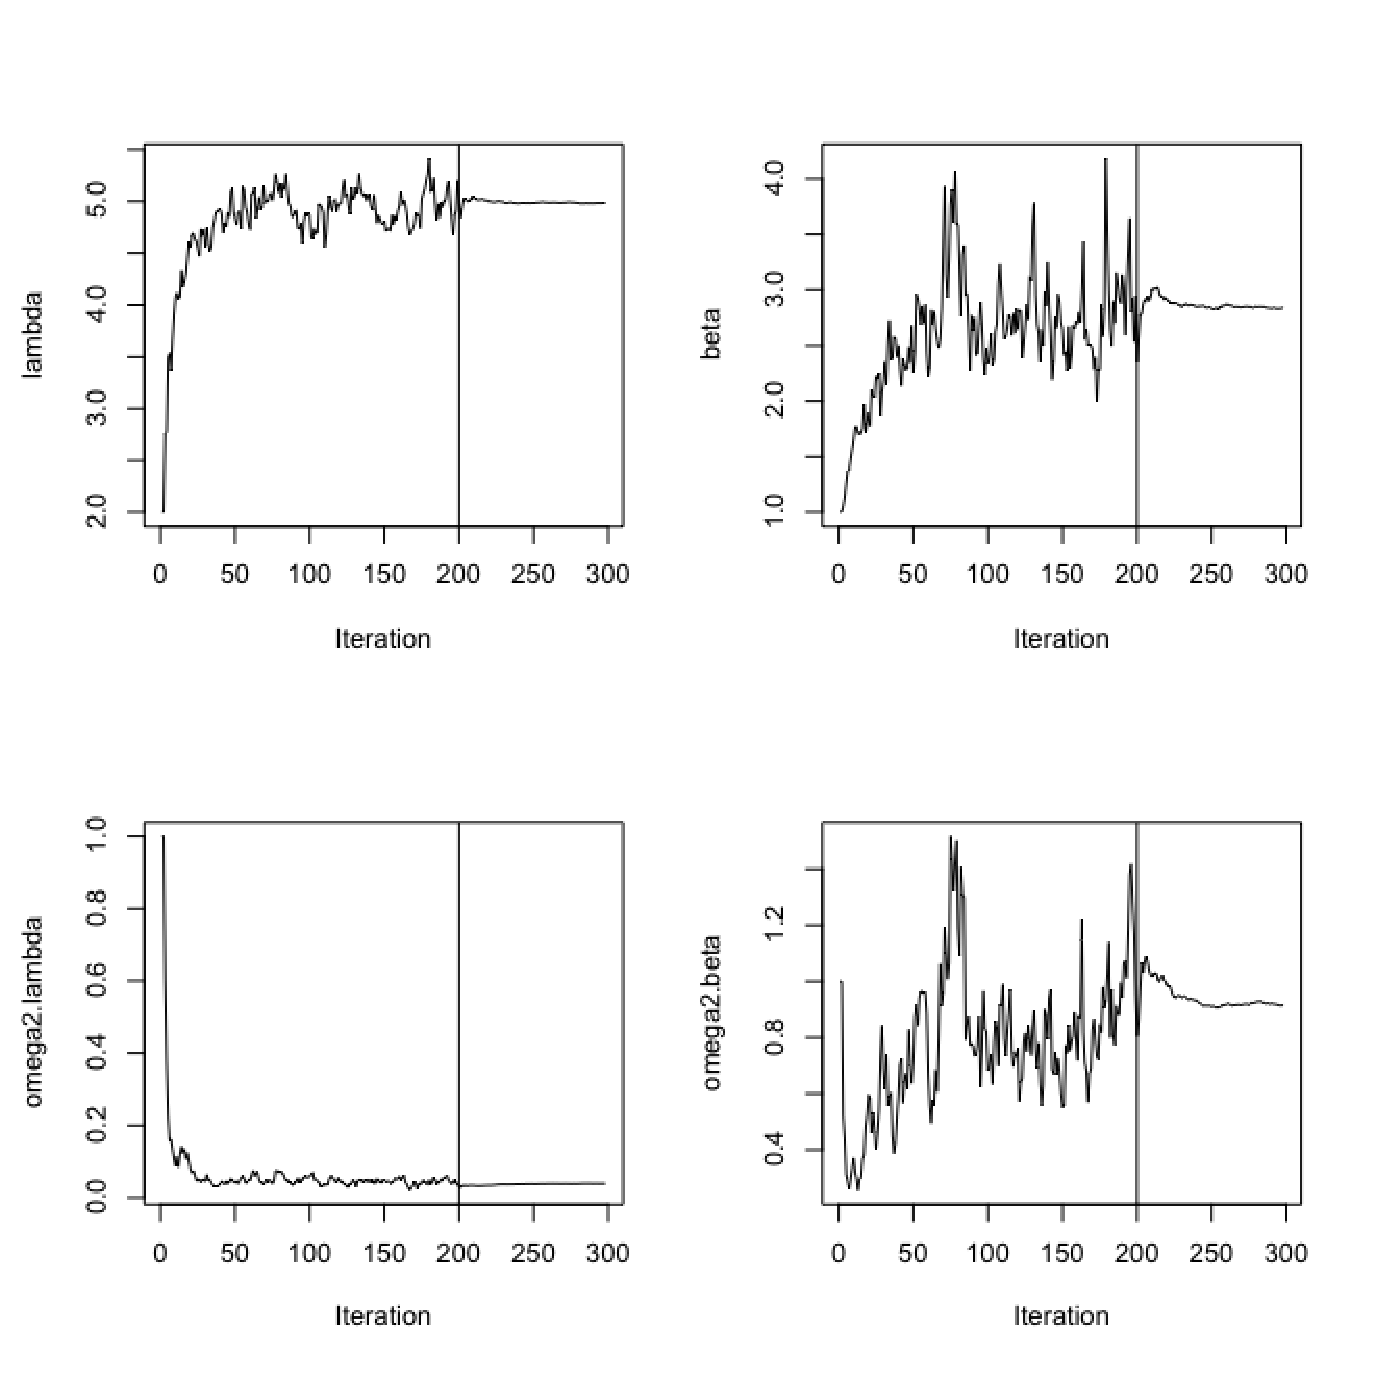
\epsfig{file=figs/popparam_tte.eps,width=12cm,angle=0}
\end{center}
\par \kern -0.5cm
\caption{Convergence plot obtained for the RTTE data} \label{fig:popTTE}
\end{figure}

